\documentclass[finalversion]{usetex-v1}

%% For intial submission uncomment the following code to remove ednote
%% comments

%\makeatletter{}
%\newsavebox{\kfl@discard}
%\renewenvironment{ednote}[1]{\@latex@warning
%  {Leftover ednote environment in final version ignored}%
%  \begin{lrbox}{\kfl@discard}}{\end{lrbox}}
%\makeatother{}

\usepackage{preamble}


\usepackage{hyperref}
\hypersetup{pdftitle = {mGTK: An \sml binding of \gtk},
            pdfauthor = {Ken Friis Larsen \& Henning Niss},
            pdfsubject = {Describtion of a Standard ML language
              binding for the graphical toolkit \gtk.},
            pdfstartview = {FitH}
            }


% Hacks
\setcounter{secnumdepth}{1}
\newcommand*{\andshare}{\end{tabular}\\\begin{tabular}[t]{c}}



\begin{document}

\title{mGTK: An \sml binding of \gtk}%\\\relax[Extended Abstract]}

\docstatus{Submitted to USENIX'04 (FREENIX track)}

\author{
\authname{Ken Friis Larsen}
\authurl{\url{ken@friislarsen.net}}
\and
\authname{Henning Niss}
\authurl{\url{hniss@it.edu}}
%
\andshare{}
\authaddr{Department of Innovation}
\authaddr{IT University of Copenhagen}
\authaddr{Denmark}
%
} % end author

\maketitle

\DefineShortVerb{\!}

\begin{abstract}
  
  We describe \mgtk, a Standard ML language binding for the
  \gtk toolkit.  \gtk is a graphical toolkit for the X
  Window System, and provides an object-oriented C language
  API.  Since Standard~ML is a mostly-functional language
  without object types, constructing a binding to \gtk is
  not a trivial task.  In \mgtk, a single-inheritance class
  hierarchy is encoded using \sml's type system. Most of the
  \mgtk binding is machine generated,  to best
  utilize the limited manpower of the project.
  
  The goal of the \mgtk project is ``just'' to present a
  type-safe interface to \gtk for \sml programmers.  This
  contrasts with GUI libraries for functional languages,
  which concentrate on producing good user interfaces: there
  are several \sml graphical user interface libraries
  available for this task.  With \mgtk, \sml applications
  have access to the mature, complete and familiar \gtk user
  interface.

%% FIXME
%%   \begin{ednote}{Bart}
%%     You will also want to add a few sentences, describing the
%%   rest of the paper contents, and describing impacts and contributions
%%   of the work.
%%   \end{ednote}

\end{abstract}



\section{Introduction}
\label{sec:intr-backgr}

%This section gives a brief introduction to \sml and \gtk, and presents
%an overview of the rest of the paper.
%
A good Standard~ML (\sml) binding to \gtk is an advantage for
both the \sml community and for the \gtk community.  The \sml
community benefits in a couple of ways. First, \sml programmers get
access to a good general-purpose graphical user interface (GUI)
library with a large range of modern widgets: the \sml community
is sorely missing such a library.  Second, it is a step in providing full access
to the whole GNOME platform. This will make it possible for \sml
programmers to make real applications without having to invent add-hoc
solutions to many standard problems, such as database access.
There are also a couple of advantages of an \sml binding
to the \gtk community. First, such a binding can help open up the small,
but important, market of teaching languages.  Second, as \sml is a
radically different language than C, an \sml binding will test the
``interfaceability'' of \gtk. This is an important design goal for the
\gtk developers.



\subsection{Standard ML}


\sml is a functional language with imperative features which is
widely used for teaching and research.  It is roughly on the same
level of abstraction as Python and Scheme. In contrast to Python and
Scheme, which are \emph{dynamically typed}, \sml is \emph{statically
  typed}, like Java and C++. This means that type errors are detected
at \emph{compile time} rather than at \emph{run time}.  Despite 
static typing, it is not necessary for the \sml programmer to
explicitly provide type annotations in the program. \sml features
\emph{type inference}: the compiler reconstructs type
annotations as needed.

\sml is one of the few languages with a formal definition.
The definition of \sml \cite{Milner:1997:Definition}
consists of 93
pages of mathematical notation (a "big step" structured operational
semantics, plus type inference rules) and English prose.  The book is
not meant as tutorial for the language. Rather, it provides an
implementation independent formulation of \sml.  This formal
definition means that it is possible to write substantial applications
in \sml that are not dependent on a specific compiler.  There are also
several mature \sml implementations with widely different
implementation strategies, ranging from byte-code interpreters with
interactive \emph{read--eval--print--loops} to aggressive
whole-program optimizing native code compilers.




\subsection{\gtk}
\label{sec:gtk}


\gtk, The GIMP Toolkit \cite{Gtk-webpage:2004}, is an LGPL-licensed
\cite{LGPL:1999} library for creating graphical
user interfaces.  It works on many UNIX-like platforms, on Windows, and
on Linux framebuffer devices.  \gtk is the graphical toolkit used in
the \gnome desktop environment. \gtk is implemented in C, with an object-oriented
hierarchy of user interface elements (``widgets''). From the beginning,
the \gtk developers have paid attention to making it feasible and
practical to develop ``bindings'' or ``wrappers'' permitting
\gtk use by programs written in
programming languages other than C. See
\cite{Gtk-bindings-webpage:2004} for a current list of bindings.

The \gtk library itself only contains widgets, but it is built on a
number of useful libraries, with which it is often
associated. Specific libraries
used by \gtk are~\cite{gtk-reference-manual}:
\begin{description}
\item[GLib] A general-purpose utility library, not specific to
  graphical user interfaces. GLib provides many useful data types,
  macros, type conversions, string utilities, file utilities, and so
  forth.

\item[Pango] A library for internationalized text handling. It
  provides the rendering engine for the widgets in \gtk that displays
  text.

\item[ATK] The Accessibility Toolkit. It provides a set of generic
  interfaces allowing accessibility technologies to interact with a
  graphical user interface.  \gtk widgets have built-in support for
  accessibility using the ATK framework.

\item[GDK] The abstraction layer that allows GTK+ to support multiple
  windowing systems.
\end{description}
Our work, however, is concentrated on the widget set itself.


%% FIXME
%% \begin{ednote}{Bart}
%%      "It is the graphical toolkit used in the GNOME platform."  Add more
%%    sentences to this to make a paragraph with a brief history of
%%    GIMP/GNOME/Gtk/Gtk+.
%% \end{ednote}

%% \begin{ednote}{Bart}
%%      "...than C."  Should section 4 material move here to
%%    describe the gtk.defs file?
%% \end{ednote}



\subsection{Overview of this paper}
\label{sec:overview-this-paper}

The rest of this paper is organized as follows.
Section~\ref{sec:brief-intr-sml} gives a brief introduction to \sml.
Section~\ref{sec:example} shows a ``Hello World'' example using \mgtk.
Section~\ref{sec:encoding-classes} explains how a single-inheritance
class-hierarchy, in particular \gtk's, can be encoded in \sml's type
system, while retaining type safety.  Section~\ref{sec:process}
describes the way that the \mgtk library is built upon the
\mgtk infrastructure.
Section~\ref{sec:mgtk-binding} describes practical matters of \mgtk,
such as which \sml compilers are supported.  Finally,
Section~\ref{sec:related-work} lists related work and
Section~\ref{sec:conclusion} gives some conclusions.



\section{Brief Introduction to \sml{}}
\label{sec:brief-intr-sml}

This section gives a brief overview of some of the main features of
\sml{}.  It is not sufficient to serve as a standalone user
programming guide for the language.
However, it should be sufficient to get an understanding of the examples in
the rest of the paper.  For more
information about \sml{}, we refer the interested reader to one of the
many fine textbooks \cite{Hansen-Rischel:1999,Paulson:1996}
available.

%% \begin{ednote}{HN}
%% I don't like the sentence ``\ldots use the language in anger'' (what
%% does this ``anger''-thing mean?).
%% \end{ednote}

%% \begin{ednote}{Ken}
%%   It mean something like ``use it for real work''.  See fx 
%%   http://homepages.inf.ed.ac.uk/wadler/papers/sigplan-angry/sigplan-angry.ps
%%   for a good explaination.
%% \end{ednote}

\sml{} is a two-level language. It consists of a \emph{core language}
for programming in the small (that is, functions, data structures and
algorithms), and a \emph{module language} for programming in the large.


\begin{figure*}[thp]
\mbox{}\hfill{}

\begin{subfloat}
\begin{minipage}[b]{.46\linewidth}
\begin{verbatim}
signature STACK = sig 
  type 'a stack
  exception EmptyStack
  val empty : 'a stack
  val push  : 'a * 'a stack -> 'a stack
  val pop   : 'a stack -> 'a * 'a stack
end
\end{verbatim}
\end{minipage}
\caption{\label{fig:stack-sig}interface}
\end{subfloat}
\qquad
\begin{subfloat}
\begin{minipage}[b]{.46\linewidth}
\begin{verbatim}
structure Stack :> STACK =
struct
  datatype 'a stack =
           Empty
         | Stack of 'a * 'a stack
  exception EmptyStack
  val empty = Empty
  fun push(elem, stack) = 
      Stack(elem, stack)
  fun pop stack =
      case stack of
          Empty => raise EmptyStack
        | Stack(top, rest) => 
          (top, rest)
end
\end{verbatim}
\end{minipage}
\caption{\label{fig:stack-struct}implementation}
\end{subfloat}
\hfill\mbox{}
\caption{Simple stack library implemented in SML.}
  \label{fig:stack-lib}
\end{figure*}

Figure~\ref{fig:stack-lib} shows a small stack library implemented in
SML.  This example shows most of the important features of SML.  The
library consists of two parts: an interface description, which is
called a \emph{signature} in SML (Figure~\ref{fig:stack-sig}), and an
implementation module, which is called a \emph{structure} in SML
(Figure~\ref{fig:stack-struct}).  Informally speaking, a
signature is the ``type'' of a structure. It specifies the
declarations of the structure that are to be externally visible.


The signature is named !STACK!. Its extent is delimited by
\texttt{sig} \ldots\ \texttt{end}. It contains five
specifications: one type specification, one exception specification,
and three value specifications.

The type specification !type 'a stack! states the
constraints on a module that
satisfies (implements) the signature !STACK!. Such a module must declare a type named
!stack!: this type is parameterized.  The !'a! is a \emph{type
  variable}: Type
variables can be instantiated to other types. This is what
is meant by a parameterized type.    Thus, the type of a
stack of integers is !int stack!, the type of a stack of integer
stacks is !int stack stack!, and so on. Type variables are at the core of
\emph{parametric polymorphism} (similar to generics in, for
example, C++ and Java; see \cite{garcia03:generics} for a comparison
of programming languages with support for parametric polymorphism).
Note that the type specification does not say anything about how a stack must be
implemented.

The exception specification states that an exception named
!EmptyStack! must be declared.

The first value specification says that a constant named !empty! must
be declared and that this constant must have type !'a stack!.  That
is, !empty! is a \emph{polymorphic} value: it can be used in contexts
where an \texttt{int stack} is needed or in contexts where a
!int stack stack! is needed.  The next value specification states that a
function named !push! must be implemented.  This function
takes two arguments, an element and a stack, and returns a stack.
Again, we see how type variables are used to specify that !push! must
work with stacks, whereas the elements can have any type.  The last value
specification states that a function named !pop! must be implemented,
and that !pop!  takes a stack as argument and returns an element and a
new stack.

Figure~\ref{fig:stack-struct} shows the code of the
implementation, in the form of a
structure declaration.  The declarations states
that the structure is named !Stack!, that !Stack! satisfies the
signature !STACK!, and that !Stack! does not reveal any implementation
details not revealed by !STACK! (the latter connoted by !:>!).  The
extent of a structure is delimited by \texttt{struct} \ldots\ 
\texttt{end}.

The parameterized type !stack! is implemented by an algebraic data
type described by a !datatype! declaration.  This declaration says that
an !'a stack! is either the constant !Empty!, or is built by
applying the constructor !Stack! to an element and a stack. (Constants
declared by a !datatype! declaration such as !Empty! are
known as constructors).

The exception declaration !exception EmptyStack! declares an
exception.

The next declaration states that !empty! is bound to !Empty!.  The
function !push! just applies the constructor !Stack! to its arguments.
The function !pop! is more interesting. This function takes a stack as argument
and then uses a !case! expression to analyze its argument.  (Here we have reused the name !stack!. Types and values uses
different name spaces: thus, the same name can be used for both a type
and a value.) 
If the argument is the empty stack (the constant !Empty!) then the
exception !EmptyStack! is raised (thrown). Otherwise, the argument
has been constructed by applying !Stack! to the arguments !top! and
!rest!, and then a pair consisting of !top! and !rest! is returned.

Users of this library can call functions from the structure
!Stack! by using ``dot-notation'': for example, !Stack.pop mystack!.

This small example illustrates one of the cornerstones in functional
programming: new values are constructed by analyzing,
composing, and sharing old values. This is in contrast to imperative and
object-oriented programming, where values are copied and modified.
(A new trend in object-oriented programming is to simulate a
functional style. See for example \cite[Item 13 and
14]{bloch01:effective-java}.)





%  \sml also features algebraic
%datatypes, pattern-matching, tuples and records, first-class and
%anonymous functions, exception handling, immutable data types and
%updatable references, abstract data types, and parametric modules, but
%it is outside the scope of this paper to introduce all these features,
%instead 





\section{``Hello World'' in \mgtk}
\label{sec:example}

Figure~\ref{fig:hello-world} shows a deliberately simple ``Hello World''
example using \mgtk. It illustrates (1)~how to get the toolkit
initialized using \texttt{GtkBasis.init} (from a module containing
basic \gtk functionality not related to specific widgets), (2)~how to
construct new widgets (using module \texttt{Window} for the Window
widget, and \texttt{Button} for the Button widget), and (3)~how to
connect signals to widgets (using module \texttt{Signal}).

\begin{figure*}[htp]
\begin{centering}
\begin{verbatim}
structure HelloWorld = struct
  fun hello _ = print "Hello World\n"

  fun main _ =
      let val _ = GtkBasis.init(CommandLine.name()::CommandLine.arguments())
          val window = Window.new ()
          val button = Button.new_with_label "Hello World"
      in  Signal.connect window (Widget.delete_event_sig (fn _ => false))
        ; Signal.connect window (Widget.destroy_sig GtkBasis.main_quit)
        ; Signal.connect button (Button.clicked_sig hello)
        ; Container.add window button
        ; Widget.show_all window
        ; GtkBasis.main() 
      end
end

val _ = HelloWorld.main()
\end{verbatim}
\caption{Hello World in \mgtk.\label{fig:hello-world}}
\end{centering}
\end{figure*}

Even this small example shows some of the main advantages of
combining \sml with \gtk.  There are no type annotations
in the program source. Nonetheless, the program is statically type-checked by
the compiler: type errors are found and reported at compile time
rather than at runtime.  In the figure we use a \sml construct
not explained earlier: the expression !fn _ => false!  denotes an
\emph{anonymous function} that returns !false! regardless of what
argument is given (you can use the \emph{wildcard pattern} !_!
(underscore) to ignore an argument to a function).
Anonymous functions are often handy for simple
callbacks, such as this one.

The construct \texttt{let}~\texttt{val}
\textit{x} \texttt{=} \textit{exp} declares the identifier \textit{x}
to be bound to the value obtained by evaluating the expression
\textit{exp}.  If the only reason for evaluating \textit{exp} is for
its side effect, one can use the wildcard pattern !_! instead of \textit{x}.
Expressions evaluated only for their side effects can also be
sequentialized using \texttt{;}.  The value \texttt{()}, the nullary
tuple of type \texttt{unit}, can be used as the return value of purely
side-effecting functions.
Such syntacic conveniences improve the readability and
quality of code.

Finally, in \sml, the double-colon \texttt{::}
denotes the cons operation on lists.  That is, to add an element $x$
to the beginning of a list $\mathit{xs}$ we write $x \texttt{::}
\mathit{xs}$ (in contrast to C++ where double-colon is the module operator).  
Built-in data types such as lists make GUI programming more convenient.

%% FIXME
%% \begin{ednote}{Bart}
%%    Explicitly say at some point that "The type of an object in
%%    a programming language is defined by the set of values it
%%    can contain."  This makes the par on base types clearer in
%%    my opinion.
%%
%%    Give examples of building up derived types from base types:
%%    in particular, you need to talk about type definitions
%%    explicitly sometime before section 3.
%% \end{ednote}


%% Example base types are {\tUnit} for the unit value \texttt{()},
%% {\tInt} for integer values, and {\tBool} for boolean values. The type
%% of a list of integers is \tList{\tInt}. The type of a function
%% expecting an integer list argument and returning an integer result is
%% \tArrow{(\tList\tInt)}{\tInt}; the \textit{length} function on lists
%% would have such a type, for example. 

%% Some functions never need to
%% ``inspect'' (sub)parts of supplied arguments values; such functions
%% are called \emph{polymorphic}. For example, the function that just
%% returns it's argument unchanged (the ``identity function'') is
%% polymorphic; so is the function that computes the length of a list. We
%% indicate the parts of the values that are not inspected by using type
%% variables $\alpha, \beta, \ldots$ at the corresponding locations in
%% the type. For example, the type of the identity function is
%% $\tArrow{\alpha}{\alpha}$ telling us that we can apply it to any type of
%% argument, and we get back a value of the same type. The
%% \textit{length} function has type $\tArrow{\tList\alpha}{\tInt}$
%% because, regardless of the type of elements in the list (here denoted
%% $\alpha$), the function can compute the length of the list. Such type
%% variables are \emph{instantiated} to (more) specific types when we
%% apply the polymorphic function. For example, when we apply the
%% polymorphic identity function to \texttt{()} we instantiate $\alpha$
%% to {\tUnit} giving this occurrence of the function the type
%% \tArrow\tUnit\tUnit; when we apply it to \texttt{17} we instantiate
%% $\alpha$ to {\tInt} and the occurrence of the function gets type
%% \tArrow\tInt\tInt. The function is said to be (parametric) polymorphic
%% because we can apply it to arguments of many shapes.

%% Some functions never need to
%% ``inspect'' (sub)parts of supplied arguments values; such functions
%% are called \emph{parametric polymorphic}. For example, the 
%% function \textit{length} that computes the length of a list is polymorphic. We
%% indicate the parts of the values that are not inspected by using type
%% variables $\alpha, \beta, \ldots$ at the corresponding locations in
%% the type. Then the type of \textit{length} is
%%  $\tArrow{\tList\alpha}{\tInt}$
%% because, regardless of the type of elements in the list (here denoted
%% by $\alpha$), the function can compute the length of the list. Such type
%% variables are \emph{instantiated} to (more) specific types when we
%% apply the polymorphic function. For \textit{length}, when we
%% apply it to a list of booleans we instantiate $\alpha$
%% to {\tBool} giving this occurrence of the function the type
%% \tArrow{\tList\tBool}\tInt; when we apply it to a list of
%% integers  we similarly instantiate
%% $\alpha$ to {\tInt}.

\section{Encoding of Classes}
\label{sec:encoding-classes}

As described in Section~\ref{sec:intr-backgr}, \sml is a functional
language without object-oriented features, while \gtk is designed as an
object-oriented library.  This mismatch makes constructing an \sml
interface to \gtk tough \begin{ednote}{HN} I don't like ``tough''.\end{ednote}.  The most difficult problem is how to represent the
subtype relations defined by a class hierarchy in \sml's type system.
In this section, we discuss how to present a
type-safe \sml interface to the \gtk class hierarchy.  By \emph{type-safe} we
mean that when an \sml application programmer using our library
makes a type-error in calling into \gtk (calling a undefined
method on object, for instance) the \sml compiler should give a
type error at compile time.

Throughout, we shall think of class hierarchies mainly as definitions
of subtype relationships.  This ``confusion'' of classes and types is
intentional: it is standard practice in types for object
oriented programming.
We are able to take advantage of two properties of \gtk
and \sml.  First, \gtk implements only a single-inheritance
class system.
Second, \sml's type system is expressive enough
to express the subtype relations of single-inheritance class
hierarchies.

We present a general method of taking a given
object oriented class hierarchy and encoding it in the \sml
type system.  The properties of the resulting encoding are: each
class type has a corresponding \sml type; the encoding is
\emph{complete} (all typings allowed by the class
hierarchy is also allowed by the encoding); and the encoding is
\emph{sound} (all typings that is disallowed by the class
hierarchy is also disallowed by the encoding).  The last property is
also called ``type safety''.  In type-theoretic jargon, the trick is to
use parametric polymorphism and \emph{existential types} to encode
inheritance subtyping.  In particular we use \emph{phantom types} to
encode the inheritance path.


\begin{figure}[htp]
  \centering
% 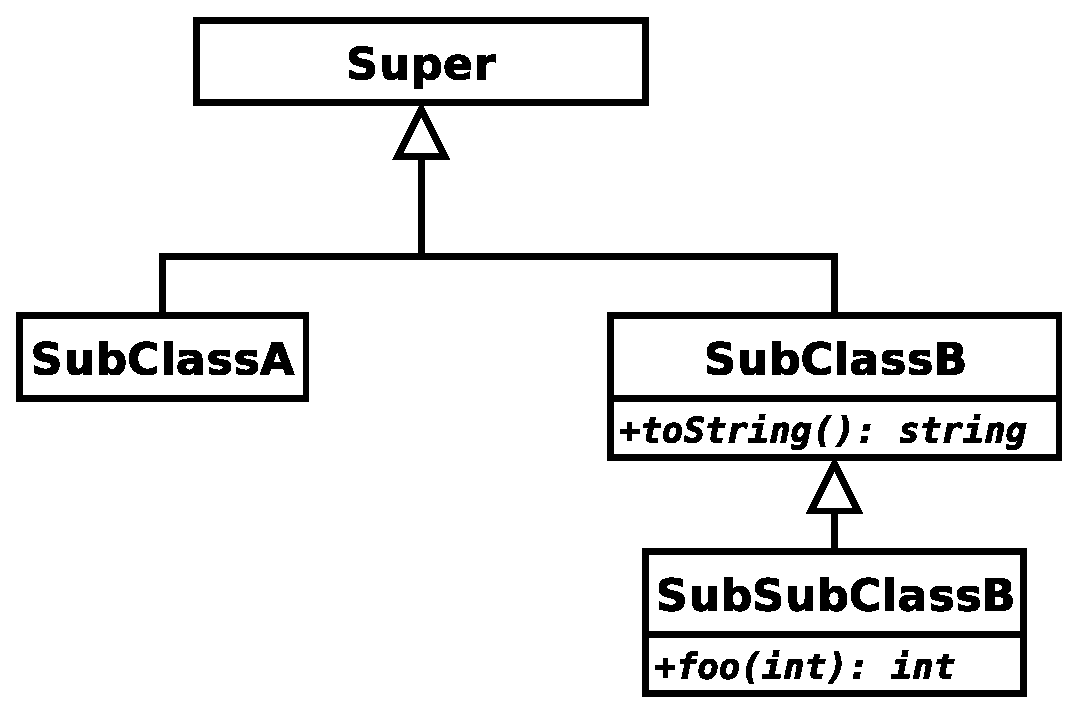
\includegraphics[width=.8\linewidth]{example-class-diagram.eps}
%  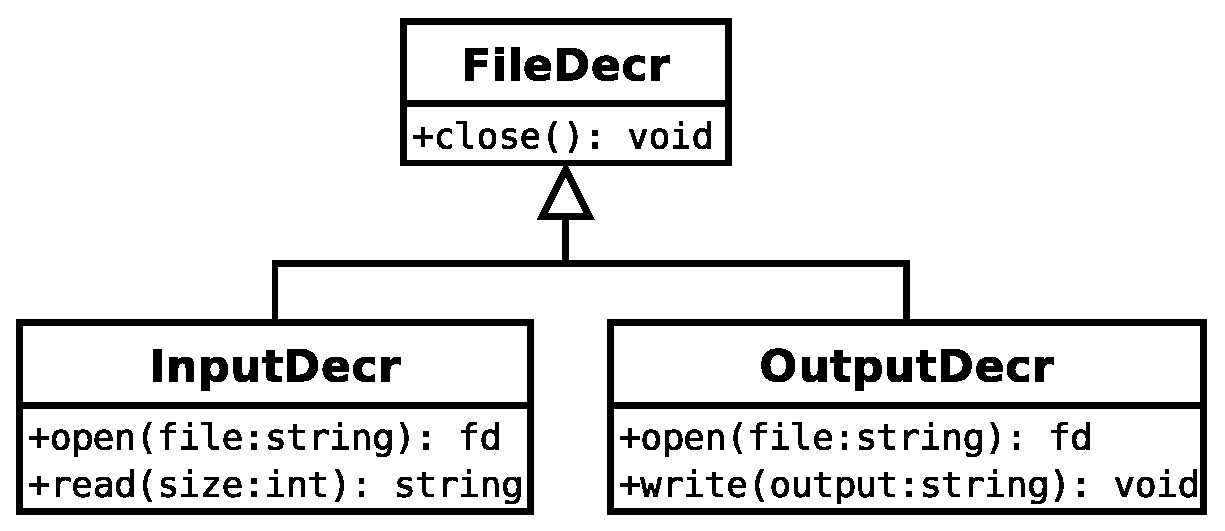
\includegraphics[width=.8\linewidth]{filedecr-class-diagram.eps}
  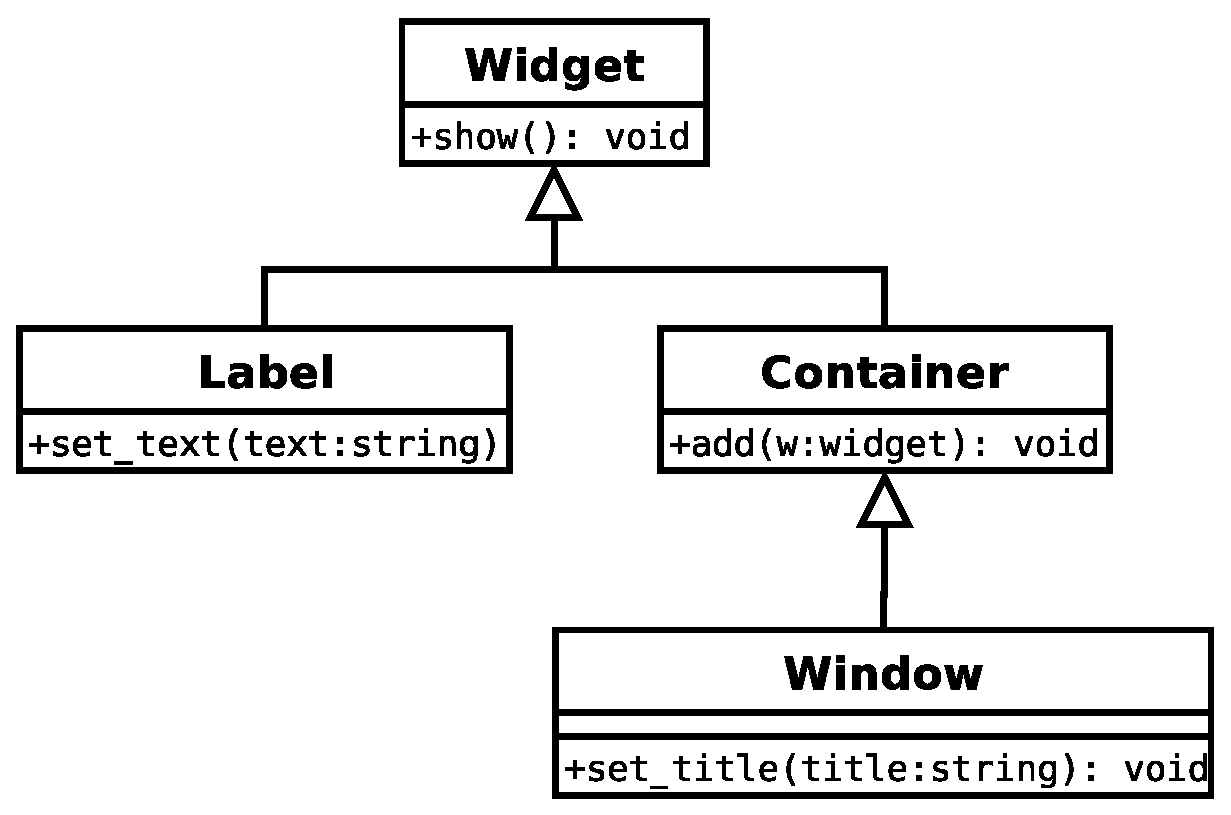
\includegraphics[width=.9\linewidth]{widget-class-diagram.mps}
  \caption{Small example class hierarchy}
  \label{fig:class-hierarchy}
\end{figure}

Figure~\ref{fig:class-hierarchy} shows a small class hierarchy with
just four classes. \classname{Label} and \classname{Container} are
subclasses of the class \classname{Widget} and \classname{Window} is a
subclass of \classname{Container}.  For the specific class hierarchy
in Figure~\ref{fig:class-hierarchy}, the properties we want to enforce
with our type encoding into \sml's type system are: that we should be
allowed to call the !show! method on all kinds of arguments whether
they are of class type \classname{Widget}, \classname{Label},
\classname{Container}, or \classname{Window}; that we should be
allowed to call the !add! method on \classname{Container}s and
\classname{Window}s, but not \classname{Widget}s and
\classname{Label}s; that we should only be allowed to call !set_title!
on \classname{Window}s; and so on.

We now describe the details of the encoding of a class.
Throughout this description we only present the \sml specifications,
that is, the parts that go into the signatures. The parts that go into
the structures are not as interesting: that is simply a matter of
calling into the C runtime.

\begin{description}
\item[Class types] A base class like \classname{Widget} in
  Figure~\ref{fig:class-hierarchy} is encoded as an abstract
  parameterized type:
\begin{SMLcode}
type 'path widget
\end{SMLcode}
(We follow the convention suggested by the \smlbasis and spell
type-names in lower-case, with underscores if needed.)  The type
variable !'path! will be used to hold the inheritance path for
subclasses.


\item[Subtyping/Inheritance] For a subclass like \classname{Label} we
  need to encode two things: the existence of the class
  (type), and the
  subtype relation to the parent class.  To do this, we declare two
  new \sml types: an abstract parameterized type, and a type
  abbreviation for specifying the inheritance.
\begin{SMLcode}
type 'path label_t
type 'path label = 
        'path label_t widget
\end{SMLcode}
We call the abstract type (here !label_t!) the \emph{witness type}
because it witnesses that the class exists.  Similar, the type !label!
is the type abbreviation that specifies that \classname{Label} inherits
from \classname{Widget}.  In the declaration of !label!  we see that
the type variable !'path! in the declaration of the type !widget!  has
been instantiated with the type expression !'path label_t!, which
contains a new type variable (also named !'path!).
In the rest of the paper we shall use the convention that witness
types ends with !_t!.

This is the juicy bit of the encoding, because this is really what
makes it possible to encode single-inheritance class hierarchies in
\sml.  Unfortunately, this is also the hardest part of the encoding to
understand.  Our experience is that you have to work a bit with some
code to really comprehend the trick.


%% \begin{ednote}{Bart}
%%   Note in particular that typing the running example into ML will
%%   result in an error, since type specifications are available only in
%%   signatures.  This is a bit confusing to even a knowledgeable reader
%%   (e.g. me :-).
%% \end{ednote}

\item[Methods] Because \sml is not an object-oriented language we shall
  model methods with ordinary functions. We use the usual convention
  that the first argument is the object on which the method is called.
  (\gtk also uses this convention.)
  
  We can now write the type for the method !add! in
  \classname{Container}:
\begin{SMLcode}
val add : 'path container -> 'a widget 
                               -> unit
\end{SMLcode}
This specification says that !add! takes two arguments, an object of type
\classname{Container} and a widget, and that it returns !unit! as result.
Similarly,  the method !set_title! from class
\classname{Window} has the type:
\begin{SMLcode}
val set_title : 'path window -> string 
                               -> unit
\end{SMLcode}
That is, !set_title! takes two arguments, an object of type 
\classname{Window} and a string, and it returns !unit!.


\item[Constructors] We have to be a bit careful with constructors.  If
  we return a value with a polymorphic type-variable !'path!
  that holds an inheritance path that has not yet been ``plugged'',
  then we could accidentally use a super-class constructor to construct
  values that can be instantiated to the type of a sub-class.  Hence,
  we introduce the abstract dummy type !base! and use that to plug the
  type variable.  Thus, the type of the constructor for
  \classname{Label} is:
\begin{SMLcode}
type base
val new : unit -> base label
\end{SMLcode}
The convention in \gtk is that constructors are named !new!.

\item[Fields] We are not able to handle fields directly, because we
  keep the representation of objects completely opaque.  Thus, all
  inspections of and changes to fields must be done through accessor
  methods.

\end{description}

We then wrap all parts of the encoding of a class into a
 signature/structure
 pair of its own.  That is, for the class \classname{Window}
in Figure~\ref{fig:class-hierarchy} the \sml signature is:
\begin{SMLcode}
signature Window =
sig
  type 'path window_t
  type 'path window = 
      'path window_t Container.container
  val new : unit -> GtkBasis.base window
  val set_title : 'path window -> string 
                                 -> unit
end
\end{SMLcode}
We see that this signature relies on two structures:
!Container! for the class \classname{Container}, and !GtkBasis! for the dummy
type !base!.  In addition to the signature !Window! we also need a
structure called !Window! that implements the actual calls to the
relevant \gtk C functions.

Does this encoding really allow all the things that the \gtk class
hierarchy allows?  Yes. For example, the function
\texttt{Container.add} has type:
\begin{SMLcode}
val add : 'p1 container -> 'p2 widget 
                                 -> unit
\end{SMLcode}
From this type we can see that, if !label! is a value of type 
%
!base label! 
% 
and !window! is a value of type !base window! then
the application
%
!Container.add window label!
%
is well-typed because: (1)~the type of !window! is just a abbreviation for 
%
!base window_t container!,
%
thus, the type variable !'p1! can be instantiated to 
%
!base window_t!,
% 
and (2)~the type of !label! is just an abbreviation of 
%
!base label_t widget!,
%
thus, the type variable !'p2! can be instantiated to 
%
!base label_t!.

Consider now the function !set_title! that only works on \classname{Window}s:
\begin{SMLcode}
val set_title : 'p window -> string -> unit
\end{SMLcode}
If we, by mistake, attempt to use this function to set the text of the
label !label! (with type !base label!) as in expression
%
!Window.set_title label "New text"!, 
%
we get a (compile-time) type error saying (essentially) that the
\classname{Label} widget is not a subclass of the \classname{Window}
widget because the inheritance paths do not match.  Here is the
concrete error message given by the Moscow ML compiler:
\begin{verbatim}
- Window.set_title label "New text";
! Toplevel input:
! Window.set_title label "New text";
!                  ^^^^^
! Type clash: expression of type
!   base label_t widget
! cannot have type
!   'a window_t container_t widget
\end{verbatim}

Hence, we have demonstrated that for these concrete
examples our encoding is both sound and complete.

%% \begin{ednote}{Ken}
%%   Explain the cool signal thing.
%%   (drop for extended abstract)
%% \end{ednote}

%% \begin{ednote}{Ken}
%%   How about the implementation of the binding with finalizers and all?
%% \end{ednote}


\section{Process}
\label{sec:process}

In constructing the \mgtk binding we leverage the foresightedness of
the \gtk developers. Early on, they recognized that it would be
important to have a machine-readable ``specification'' of the toolkit.
The specification would describe the widget classes, the
inheritance hierarchy, and methods and functions in the toolkit. This
specification was implemented using a lisp-like custom notation in the
\texttt{gtk.defs} file of the toolkit. One could
argue that it is simple enough to extract the same information from
the C header files. However, C headers are difficult to parse, whereas
the defs format is straightforward to parse.

The bulk of the \mgtk binding is constructed automatically from the
\texttt{gtk.defs} file.  The complete binding process is naturally
divided into two phases: (1) binding design, where we apply the
principles described in Section~\ref{sec:encoding-classes} to a few
representative widgets to demonstrate the structure of the binding,
and (2) binding construction, where the structure in (1) is applied to
the entire toolkit. It is important to note here that the design phase
can be carried out for a very small subset of the toolkit, after which
the construction phase ``mimics'' that for the complete toolkit.
% We refer to the design as a
%\emph{muck-up} and the result as \minimgtk.

This phase separation makes it easier to get the design right, simply
because there are fewer issues to deal with.  It also makes the work
involved in moving the binding to other \sml compilers manageable:
the compiler writers can provide the equivalent
of the small subset for their compiler, and utilize that style during the
construction phase. We also hope that the phase separation will help when new releases
of \gtk are produced. Most of the work in constructing the binding for
the new release is over when the design of the small subset has been
completed.

Let us return to our running example, and look at some example
specifications of widgets, functions/methods, and signals.
Figure~\ref{fig:gtk-defs} shows three entries in the \texttt{gtk.defs}
file.
\begin{figure}[htbp]
\begin{centering}
\begin{verbatim}
(define-object Container
  (in-module "Gtk")
  (parent "GtkWidget")
  (c-name "GtkContainer")
  (gtype-id "GTK_TYPE_CONTAINER")
)

(define-method gtk_container_add
  (of-object "GtkContainer")
  (c-name "gtk_container_add")
  (return-type "none")
  (parameters
    '("GtkWidget*" "widget")
  )
)

(define-signal delete-event
  (of-object "GtkWidget")
  (return-type "gboolean")
  (when "last")
  (parameters
    '("GdkEventAny*" "p0")
  )
)
\end{verbatim}
\caption{\texttt{gtk.defs} excerpt.\label{fig:gtk-defs}}
\end{centering}
\end{figure}
The first entry shows a widget specification indicated by
!define-object!. From the entry we see that the !GtkContainer! widget
(the name appearing right after !define-object! is a shorthand)
inherits from !GtkWidget!, and it belongs in the !Gtk! module.  We also
see the type assigned to instances of this widget in the \emph{\gtk type
system} (which is completely unrelated to the \sml encoding given
above).

The next entry shows a method specification for the method !add!.
This method takes a !GtkWidget*! (in the C implementation)
argument, and returns nothing. Since it is a method, there is an
implicit ``self'' argument of type !GtkContainer*!.

The final entry shows a ``signal handler'' or (``callback'')
specification. In this case, we specify the prototype for handlers of
delete events on widgets. The signal handler for !delete-event! for
widget !GtkWidgets! accepts a parameter of type !GdkEventAny*!, and
returns a value of type !gboolean!. 

%\subsection{Stubs and code generation}
%\label{sec:stubs-code-gener}


%% \section{Synergy}
%% \label{sec:synergy}

%% \begin{ednote}{Henning}
%%   SML + Gtk+ er godt
%%   (drop for extended abstract?)
%% \end{ednote}



%% \section{Supported \sml compilers}
%% \label{sec:supp-sml-comp}

%% \begin{ednote}{Henning}
%%   MLton og Moscow ML (SML.NET med Gtk\#?)
%% \end{ednote}

\section{The \mgtk Binding}
\label{sec:mgtk-binding}

The \mgtk binding is available at SourceForge \texttt{http://mgtk.sf.net/}
and is released under the GNU Lesser General Public License
(LGPL) \cite{LGPL:1999}.

A fundamental difference in producing \sml bindings of \gtk, compared
to bindings for other languages, is the existence of a variety of
compilers (Section~\ref{sec:intr-backgr}). This sets
this work apart from bindings to languages such as Python, where
there is only one target compiler and runtime system. 

The encoding of the \gtk class hierarchy in the \sml type system in
Section~\ref{sec:encoding-classes} is \emph{the} core aspect of the
binding. As the encoding stays within the language as defined in the
Definition~\cite{Milner:1997:Definition}, this aspect of the binding
remains the same for all \sml compilers conforming to the Definition.
In other words, the interface exposed to the application programmer is
the same across all compilers.
%
One finds \sml and \gtk implementations on a large variety of
platforms. Thus, the GUI porting work in moving application programs from one of these
platforms to another is largely eliminated. \begin{ednote}{HN} is this not too understated? \end{ednote}

The \mgtk binding already targets two of the main \sml systems,
\mosml~\cite{Mosml-webpage:2003} and \mlton~\cite{MLton-webpage:2003}.
The authors are currently looking into constructing
bindings for other \sml compilers (in particular, the \emph{ML Kit
  with Regions} \cite{MLKit-webpage:2003} and \emph{SML.NET}
\cite{SML.NET-webpage:2003} with \gtksharp). As mentioned earlier
(Section~\ref{sec:process}), the issues here  mainly involve interfacing
to C.

The potential for partial compiler independence sets the present binding
apart from other \gtk bindings for \sml; notably, the \texttt{SML-Gtk}
binding for the \sml of New Jersey compiler
\cite{SML-Gtk-webpage:2003}.  The \texttt{SML-Gtk} binding is also based
on phantom types. Our binding predates the \texttt{SML-Gtk} binding by
approximately two years---the \texttt{SML-Gtk} User's Manual refers to the
\mgtk binding.  To date no serious attempts has been made to merge
these two projects.  The reason for this is that, even though
the projects seems similar, we have followed rather different
strategies for constructing our respective bindings.  \texttt{SML-Gtk}
is partly generated by the !ml-nlffi! foreign function interface, for instance, and does not attempt to
automate memory management.

%% \begin{ednote}{Bart}
%%   This work vs SML/NJ?  Is this a replacement for Leung's
%% system?  You need to cite [10] much earlier in the paper,
%% and make it clear that you are not the only ones to use
%% phantom types for this task.  In particular, I don't see how
%% the claim that "the encoding of a single inheritance
%% hierarchy as above is [new]." can be true, given that [10]
%% appears to have a very similar system.  Do you predate this
%% work?

%% \end{ednote}


\section{Related Work}
\label{sec:related-work}

The list of language bindings for \gtk shows a plethora of different
languages from which \gtk is accessible. In this section we briefly
discuss the bindings most related to \mgtk.

When considering ML-like languages, there are two major alternatives
to the \mgtk binding. The !SML-Gtk! binding was discussed earlier.
%
The !lablgtk! binding is a \gtk binding for O'Caml.
O'Caml is a ML dialect different from \sml: among other
things, it
has object-oriented features. This binding, therefore, can
directly utilize the \gtk object hierarchy.

\gtk has also been bound to other functional languages.
For example, !gtk+hs! is a Haskell binding,
% \url{http://www.cse.unsw.edu.au/~chak/haskell/gtk}
and !erlgtk! is an Erlang binding.
% \url{http://erlgtk.sourceforge.net}
%
Bindings also exist for other graphical toolkits.
For example, !sml_tk! is an \sml binding of Tk.
% \url{http://www.informatik.uni-bremen.de/~cxl/sml_tk}

The use of phantom types to express invariants about programs
is not new. However, the encoding of a single-inheritance hierarchy as
above is original with us. Independent work has established similar results
\cite{Fluet-Pucella:2002}. %
On the construction side of things, other bindings are also machine
generated. For this, some of the bindings use the \emph{Simplified
  Wrapper and Interface Generator} (SWIG)
\cite{Beazley:1996}, while others
extract appropriate information directly from the C headers files of
\gtk.

From the outset, the necessity of access to libraries has been realized
in the functional programming community. Work in this area for \sml
includes
%\mosml's C-library support \cite{Larsen:2001} and 
\smlnj's foreign function interface \cite{Blume:2001:nlffi};
for Haskell it includes \cite{Finne:1999:CallingHellFromHeaven}.



\section{Conclusions and Future Work}
\label{sec:conclusion}

It is our intention to continue this work by utilizing appropriate
programming language technology to gradually bind more and more of the
\gnome development platform for \sml. As was the case above, this
entails designing appropriate representations of the platform in the
\sml world (in particular, preserving the type-safety property mentioned
above). It also includes the more practical work of extending the code
generator to handle such newly introduced representations.

The long term goal for \mgtk is to target most of the \gnome{}
platform.  The advantages of bringing \gnome to the \sml community in
the form of such bindings are twofold. Firstly, it would allow \sml
programmers access to the vast collection of useful application-level
support in \gnome. Secondly, it would allow \sml programmers to take part in
the development of \gnome components, by allowing them to write such
components in \sml. The key technical aspect to be solved here is to
support type-safe inheritance on the \sml side of things. Of course,
one will also have to explore exactly how to tie the various languages
together.  The \gnome community already has experience in this area.

%% \begin{ednote}{Bart}
%%   Expand the discussion here substantially: it sounds
%% interesting.  What will it take to write SML-GNOME apps?
%% What parts will you replicate/replace?  What parts will you
%% just interface to?

%% \end{ednote}

In this paper we have demonstrated that it is theoretically and
practically possible to make a type-safe interface from \sml to \gtk.
This is interesting for several reasons. First, \mgtk was one of the
first graphical toolkits available to the \sml community. Second, the
fact that it is possible to make an \sml binding to \gtk
attests to the claimed ``interfaceability'' of \gtk, because \sml is so
radically different from C in abstraction level and paradigm. Third,
by auto-generating the binding, we get a binding of the complete \gtk
toolkit. Finally, we believe that the particular way we construct the
binding can be extended to bind the
entire \gnome development platform, using mainly machine generated
stub code.


\section{Acknowledgments}
\label{sec:acknowledgments}

We are grateful to the lead developer of \mosml, Peter~Sestoft, who
have answered a multitude of questions about interfacing \mosml with C
libraries.  Without Peter's initial technical support, \mgtk would
never have seen the light.  Likewise, the \mlton developers, in
particular Stephen~Weeks, has been supportive in answering questions
about interfacing \mlton to C.  They have even made changes to the \mlton
compiler that was needed for \mgtk.  Also, we would like to thank the
IT~University of Copenhagen, were we have been employed while doing the
greater moiety of the work presented in the article.  Finally, we
must express our deepest gratitude to our FREENIX shepherd on this
article, Bart~Massey.  Without his patience, encouragements, and many
suggestions for improvements, this article would have been much less
readable.


\bibliographystyle{plainnat}
\bibliography{mgtk}

\end{document}

%%% Local Variables: 
%%% mode: latex
%%% TeX-master: t
%%% TeX-command-default: "PDFLaTeX"
%%% End: 

% LocalWords:  mGTK FREENIX Friis Niss GtkBasis fn wildcard tl gtk defs SML API
% LocalWords:  GtkWidget MLton mgtk interfaceability eval REPLs LGPL GLib Pango
% LocalWords:  framebuffer ATK GDK sig EmptyStack struct datatype mystack init
% LocalWords:  nullary xs subtyping GtkContainer GtkWidgets GdkEventAny nlffi
% LocalWords:  gboolean SourceForge lablgtk O'Caml hs erlgtk Tk sml tk Sestoft
